\documentclass[tikz,border=8pt]{standalone}
\usetikzlibrary{arrows.meta,positioning}
\begin{document}
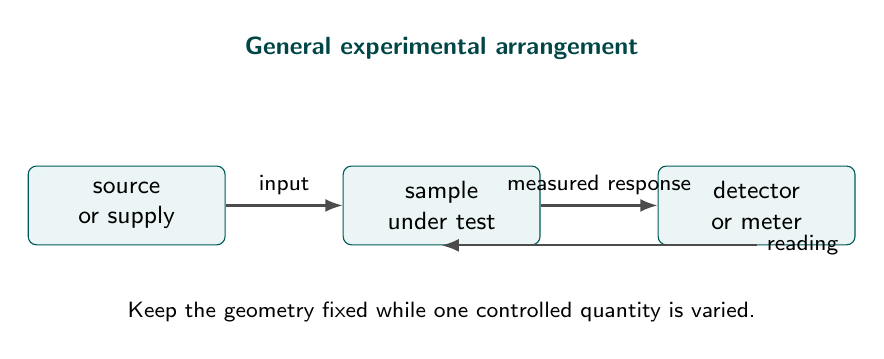
\begin{tikzpicture}[
  box/.style={draw=teal!70!black, rounded corners=3pt, fill=teal!8, minimum width=2.5cm, minimum height=1.0cm, align=center, font=\sffamily\small},
  arrow/.style={-{Latex[length=2.2mm]}, draw=black!70, line width=0.8pt},
  label/.style={font=\sffamily\bfseries\small, text=teal!55!black}
]
\node[label] at (0,2.0) {General experimental arrangement};
\node[box] (source) at (-4,0) {source\\or supply};
\node[box] (sample) at (0,0) {sample\\under test};
\node[box] (detector) at (4,0) {detector\\or meter};
\draw[arrow] (source)--node[above,font=\sffamily\footnotesize]{input} (sample);
\draw[arrow] (sample)--node[above,font=\sffamily\footnotesize]{measured response} (detector);
\draw[arrow] (detector.south) |- node[pos=0.25,right,font=\sffamily\footnotesize]{reading} (sample.south);
\node[font=\sffamily\footnotesize,align=center] at (0,-1.35) {Keep the geometry fixed while one controlled quantity is varied.};
\end{tikzpicture}
\end{document}

